\section{Case Studies}\label{sec:case-studies}

% \ds{TODO: This section is just a list of pointers. Need to write properly.}
We demonstrate the expressiveness and practicality of guardrails through multiple case studies across several OS subsystems.
We design and implement guardrails for traditional Linux policies (\Cref{subsec:cbmm-case-study,subsec:compaction-case-study}) as well as learned OS policies (\Cref{subsec:flux-case-study,subsec:mllb-case-study}). We also demonstrate how guardrails can be helpful in identifying issues with, and refining existing traditional (\Cref{subsec:arms-case-study}) and learned (\Cref{subsec:kml-case-study}) policies.
For each case study, we explain the guardrail (the run-time monitorable property and corrective action), the \perfsafety property  that the guardrail should meet, and the implementation needed to enable the monitor.

\subsection{Transparent Hugepage Promotion in CBMM}
\label{subsec:cbmm-case-study}

As described in \Cref{sec:background}, CBMM uses offline profiled benefits and compares them against an estimated cost of allocation to decide whether to promote a hugepage. 

%\paragraph{Benefit correction guardrail.}
%As described previously in \Cref{sec:background,sec:guardrails}, 
%We design the CBMM guardrail to check if the benefits between two page regions follow the same relationship as the number of accesses to them (\Cref{lst:benefit-correction}).
%This guardrail uses several primitives introduced in \Cref{tab:gdl-primitives}.
% $P_i$ and $P_j$ are page regions (and hence, of the type $Set[{\sf Page}]$).
%It uses the {\tt read(.)} primitive to get {\tt accesses} for each page region and reads the {\tt Benefit} map as a feature in the in-kernel store.
%We implement the access counts using the Damon tool~\cite{damon-middleware19}.
%The guardrail action is to set per-page-region parameters, $\Delta{\sf benefit}$, which prescribes by how much the benefit should change for a given page region. 
% As mentioned previously, the mechanism to collect the per-page-region attribute ({\tt accesses} as well as the mechanism to enforce the change in benefits (via the {\sf Set} action) must be implemented by the user.

\paragraph{Benefit correction guardrail.}
We design the CBMM guardrail to check whether the ordering of benefits across page regions matches the ordering induced by their access counts (\Cref{lst:benefit-correction}). This guardrail uses several primitives from \Cref{tab:gdl-primitives}. In particular, it uses the {\tt read(.)} primitive to obtain the {\tt accesses} value for each page region and to read the {\tt Benefit} map from the in-kernel store. We implement access counting using the Damon tool~\cite{damon-middleware19}. When the guardrail is violated, its action updates the per-page-region correction parameter $\Delta{\sf benefit}$, which determines how much the benefit estimate for that region should be adjusted.

\paragraph{Verifying \perfsafety.}
Let $a_i$ denote the recent access count of page region $P_i$, $b_i^{prev}$ denote its previous benefit estimate, $c_i$ denote its estimated promotion cost, $b_i^{true}$ denote its true runtime benefit, and $b_i^{live}$ denote the benefit estimate after correction. Then, we write the \perfsafety property, $\Phi$ as:
\[
\begin{aligned}
% \Phi_{\mathsf{NR}} \triangleq\;&
\Bigl(\forall P_i.\;& (b_i^{true} < c_i \land b_i^{prev} < c_i)
\Rightarrow b_i^{live} < c_i \Bigr) \\
&\land\;
\Bigl(\forall P_i.\; (c_i < b_i^{true} \land c_i < b_i^{prev})
\Rightarrow c_i < b_i^{live} \Bigr).
\end{aligned}
\]
% \eric{superscript means previous region.. needs something thats not confusing}
This says that for every page region whose CBMM decision was already correct, the repaired estimate must preserve that decision: pages that were correctly estimated to not be promoted still have benefits below the costs, and pages that were correctly estimated to be promoted should have benefits higher than costs.
The system model assumes the true benefit is proportional to the number of accesses, that is, \( b_i^{true} = \kappa a_i\), for $\kappa > 0$. The guardrail condition, $G$ checks whether the ordering induced by the live estimates agrees with the ordering induced by accesses:
\[
% G_{\mathsf{BC}} \triangleq
\forall P_i,P_j.\; a_i > a_j \Rightarrow b_i^{live} > b_j^{live}.
\]
Then, the corrective action is to adjust the benefit estimates so that they align with the access counts. We do so using the following adjustment for every page region $P_i$:
\[
b_i^{live} = b_i^{prev} * ((1 + a_i) / a_i^{prev})
\]
We take the guardrail's local guarantee to be exactly $\Phi$. It therefore suffices to show that, under the system model, the guardrail condition $G$ (the {\tt check} clause in \Cref{lst:benefit-correction}) implies $\Phi$, and that when $G$ fails, the update action establishes $\Phi$. Both obligations are easily discharged by Z3. Our verifier proves $\Phi$ in an average of 27\,ms over 15 runs.

\paragraph{Implementation.} 
We implement the CBMM hugepage promotion policy in Linux v6.12. In user space, the guardrail monitor periodically invokes Damon to obtain per-region access counts and uses them to compute benefit estimates, which scale linearly with the number of accesses. These estimates are then written to an in-kernel profile mapping virtual address ranges to benefits. We add kernel modules that update this profile through writes to designated proc files from user space. CBMM then uses the updated profile for subsequent promotion decisions.
% Specifically, for each interval $i \in [1 ... n]$ each period we approximate $A$, the number of access per damon reported region in the last period, set $S[i]$ and $E[i]$ to the interval endpoints, and scale $B[i]$ by $(A' + 1)/A$ where $A'$ is the number of access samples reported by damon this current period.
% A potential drawback of this approach is if the set of regions reported by damo changes drastically, however for the most part the regions remain consistent.
% Tests were run on the c220g2-010604 cloudlab node in the University of Wisconsin, on Ubuntu 24.04 running a modified version of Linux 6.12 which integrates the kernel policy and modules.

\paragraph{Results.}
We evaluate default CBMM and CBMM augmented with our guardrail on YCSB workloads over MongoDB. Each workload uses $2^{22}$ operations over $2^{22}$ records. \Cref{fig:hugepage-cbmm-plots1} shows the resulting 2.7-3.5\% throughput improvement from updating CBMM's benefit estimates using the observed access counts of page regions, as described above.
% \aditya{what is the quantitative observation or takeaway}

\begin{figure}[t!]
    \centering
    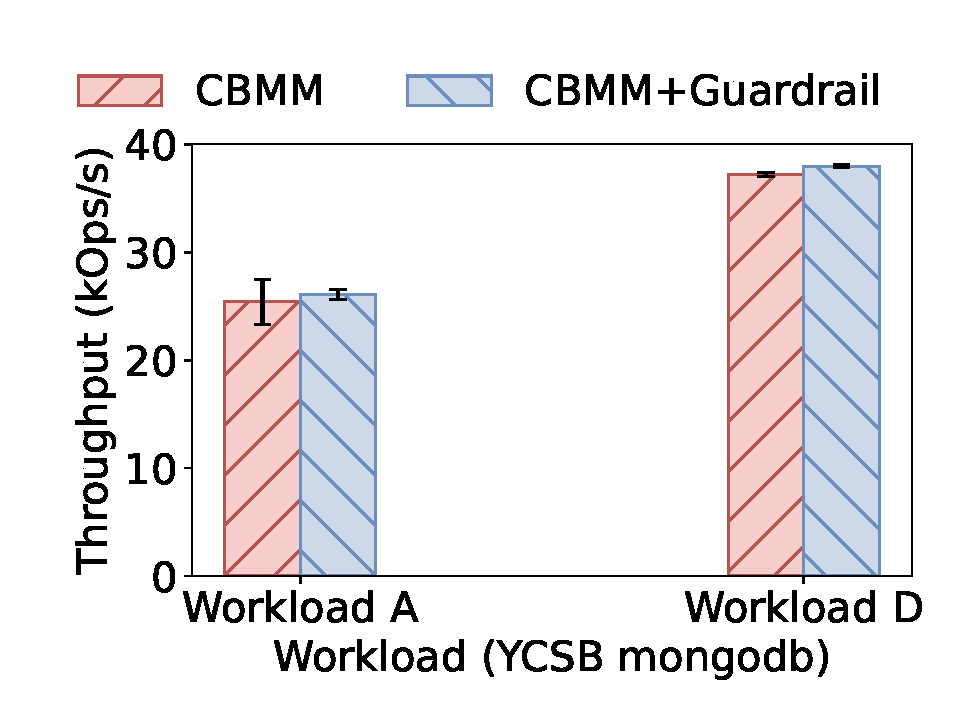
\includegraphics[width=0.58\columnwidth]{figures/CaseStudies/HugePage/cbmmplots.pdf}
    \caption{Performance of CBMM with and without guardrail.}
    \label{fig:hugepage-cbmm-plots1}
\end{figure}
% Unused: Bar chart for [workload A or D, and then (throughput, read 99p latency, update 99p latency)]. Each blob has three bars: one for CBMM, one for policy with default value 200000, one for policy with default value 21531397. Average across 4 runs.

\subsection{Memory Compaction in Linux}
\label{subsec:compaction-case-study}

The Linux kernel performs memory compaction to create physically contiguous free memory required for large allocations such as hugepages and certain device buffers.
Compaction can occur asynchronously via the {\tt kcompactd} daemon or synchronously along page allocation paths.
Whether invoked via hugepage allocation or the {\tt kcompactd} daemon, compaction is performed by invoking {\tt compact_zone()}.

\paragraph{Bounded overhead guardrail.}
While compaction improves allocation success rates and reduces fragmentation, it can incur substantial CPU overhead and stall latency under memory pressure. 
In particular, this memory pressure is elevated when hugepage allocation is enabled because of memory bloat~\cite{cbmm-atc22,ingens-osdi16}. 
Thus, we design a guardrail specifically when transparent hugepage promotion is active:
% The first is a guardrail that checks if the cost of running compaction is bounded by a threshold and if not, it temporarily switches off hugepages. The second guardrail restores hugepage allocations after waiting for a fixed duration.
%We write these guardrails in \lang as follows:
\begin{dslbox}[title={Listing~\theguardcount: Bounded overhead of memory compaction}, glabel=lst:compaction]
for THPAlways
when periodic(5s)
check $\forall e \in$ compact_zone() avg(exec_time(e)) < 30ms
action Set(thp_policy, THPNever)
\end{dslbox}

% for THPNever
% when periodic(10s)
% check True
% action Set(thp_policy, THPAlways)

% \ds{We probably need to add some syntax for guardrails to check if other guardrails are installed -- e.g., RestoreTHP by itself should not be triggered.}
The above guardrail applies only when the THP policy is {\tt THPAlways}, that is, when the Linux {\tt thp\_enabled} flag is set to {\tt always}. It checks whether the average execution time of {\tt compact\_zone()} over 5-second windows remains below 30\,ms; otherwise, the corrective action switches the policy to {\tt THPNever}. The purpose of this action is to let processes use fragmented memory regions without incurring the compaction overhead induced by hugepage allocation.
% \ds{@Sujay: I added the previous statement as an intuitive explanation. Please confirm if this statement is accurate?}

\paragraph{Verifying \perfsafety.}
% To keep the proof simple, the current \lang model formalizes only the overhead-control guardrail; the timed {\tt RestoreTHP} guardrail is omitted from this minimal verification sketch. 
Let $\policy_{\mathsf{thp}}$ denote the current THP policy, let $\mathsf{avg}(\policy)$ denote the average execution time of the kernel function {\tt compact\_zone} under $\policy$, and let $B$ denote the compaction-overhead budget. The asserted \perfsafety, $\Phi$,  is:
\[
% \Phi \triangleq
(\policy_{\mathsf{thp}} = {\tt THPAlways}) \Rightarrow \mathsf{avg}(\policy_{\mathsf{thp}}) \leq B
\]
This property says that the system is safe either because hugepage promotion is disabled, or because it remains enabled only when the measured compaction overhead is within budget.
The guardrail condition, $G$, is simply the bounded-overhead check
\(
\mathsf{avg}({\tt THPAlways}) \leq B_{\mathsf{over}},
\)
and by setting the local guarantee to be the same as the asserted property, i.e.\;
\(
\varphi := \Phi
\), the solver proves \perfsafety{} in in an average of 15.1\,ms over 15 runs.  

\paragraph{Implementation.}
We use the {\tt exec\_time} primitive in \lang for this guardrail. This is implemented via a combination of two eBPF programs attached as kprobes and kretprobes (as described in \Cref{sec:infra}) to the {\tt compact\_zone()} function.

\begin{figure}
    \centering
    \includegraphics[width=0.7\columnwidth]{figures/CaseStudies/Compaction/compaction\_tput.pdf}
    \caption{Throughput for YCSB-Redis workload when using the memory compaction guardrail.}
    \label{fig:compaction-results}
\end{figure}

\paragraph{Results.}
We first run a process that fragments a certain fraction of available memory, then run the YCSB workload over a Redis server, and measure the average throughput over five runs. \Cref{fig:compaction-results} shows that the ability of the guardrail to revert to base pages when they are not useful, leading to 0.5-6.6\% higher throughput, especially at high fragmentation.

\subsection{Learned Flow Scheduling}\label{subsec:flux-case-study}

In datacenter networks, flow scheduling is crucial in minimizing the end-to-end latency.
Prior works have shown that knowing flow sizes (the amount of bytes that a flow must send) can improve scheduling~\cite{pfabric-sigcomm13,fastpass-sigcomm14,homa-sigcomm18}.
This has also motivated investigations into learned flow size predictors~\cite{flux-nsdi19}. In practice, however, these predictors face a tension between generalization and inference cost.
While large training datasets and large models could, in principle, improve accuracy across diverse applications, predictions must be produced quickly enough to inform scheduling, limiting the model size that can be used online. As a result, small predictors may fail to generalize across heterogeneous workloads.
In this study, we build two small neural networks -- one trained on flows from long-running data-processing jobs, and another trained on flows from short echo server applications.
These two neural networks can be thought of as two different policies: {\tt FLUXShortPredictor} and {\tt FLUXLongPredictor}.

\paragraph{In-distribution check guardrail.}
As described in \Cref{fig:flux-example}, the guardrail checks the use of the correct models depending on whether a new flow's features  are in-distribution or not: %. This is expressed in \lang as:
\begin{dslbox}[title={Guardrail~\theguardcount: In-distribution checks for two flow size predictors}, glabel=lst:in-dist]
for FLUXShortPredictor
when on_call(flow_start)
check $agg\_net \sim$ read(ShortDist[agg_net]) $\wedge$
      $cpu \sim$ read(ShortDist[cpu]) $\wedge$
      $ram \sim$ read(ShortDist[ram]) $\wedge\ \dots$
action Set(flux_policy, FLUXLongPredictor)

for ${\sf FLUXLongPredictor}$
when on_call(${\sf flow\_start}$)
check $agg\_net \sim$ read(LongDist[agg_net]) $\wedge$
      $cpu \sim$ read(LongDist[cpu]) $\wedge$
      $ram \sim$ read(LongDist[ram]) $\wedge\ \dots$
action Set(flux_policy, FLUXShortPredictor)
\end{dslbox}
The above guardrails read the flow features ($agg\_net$, $cpu$, $ram$, etc.) and check whether they are from the same distribution as the training data for a given predictor.
The latter are assumed to be readable from maps {\tt ShortDist} and {\tt LongDist} for the two models.
The operator $\sim$ returns true if the probability of a value being in a distribution is above a permissible bound.
Note that when an input feature is out of distribution for either model, the outcome is non-deterministic because the guardrail cannot impose any selection. 
% \aditya{I don't understand the action. why do you switch to long when short fails -- i.e. why is that switch kosher?}
% \aditya{in- vs out-of-dist applies to non-learned policies too? likewise, does decision quality extend to non-learned?}

\paragraph{Verifying \perfsafety.} Let $\policy$ denote the current scheduling policy, let $D_{\mathsf{short}}(\vec v)$ and $D_{\mathsf{long}}(\vec v)$ denote the predicates saying that the current feature vector $\vec v$ is in distribution for the short- and long-flow predictors, respectively, and let $Q(\policy, \vec v)$ denote the predicate that policy $\policy$ will have acceptable recent decision error on flows with feature vector $\vec v$. The asserted \perfsafety property, $\Phi$, is just $Q$.

The system model assumes that there are only three policies, and the default scheduler is always of sufficient quality, that is, for every feature vector $\vec v$,
\begin{mathpar}
Q({\tt Default}, \vec v)
\end{mathpar}
and that the specialized predictors are of sufficient quality when their inputs are in distribution, that is, for  $\forall \vec v$,
\[\begin{aligned}
&D_{\mathsf{short}}(\vec v) \Rightarrow Q({\tt FLUXShortPredictor}, \vec v) \\
\wedge\;\;& D_{\mathsf{long}}(\vec v) \Rightarrow Q({\tt FLUXLongPredictor}, \vec v).
\end{aligned}\]
Once again, the local guarantee is exactly the same as the asserted property, so we set
\(
\varphi \triangleq \Phi.
\), and the guardrail conditions are exactly the in-distribution checks, so the results are easily discharged by the solver; our implementation proves $\Phi$ in an average of 19.5\,ms over 15 runs.

\paragraph{Implementation.}
We deploy these trained neural networks through a kernel--user-space pipeline. eBPF programs collect features at flow start and write them to an eBPF map. A user-space daemon then reads these features, runs neural-network inference to predict flow size, and writes the result back to a file socket that the kernel reads.

\begin{figure}
    \centering
    \includegraphics[width=0.7\columnwidth]{figures/CaseStudies/FLUX/flux\_accuracy.pdf}
    \caption{Comparison of {\tt FLUXShort} and {\tt FLUXLong} against the combination of the two under guardrails.}
    \label{fig:flux-results}
\end{figure}

\paragraph{Results.}
We test three approaches: (i) using only {\tt FLUXShort}, (ii) using only {\tt FLUXLong}, and (iii) a combination of the two protected via the in-distribution check guardrail.
For (iii), the guardrail evaluates which model must be used for each new flow, depending on whether its features are in-distribution for {\tt FLUXShort} or {\tt FLUXLong}. We evaluate these three approaches for two workloads: one with 80:20 split for short and long flows and another with 20:80 split.
\Cref{fig:flux-results} shows that by making these switches for appropriate flows, the guardrail enables good predictions (<25\% error) for more than 85\% of the samples, resulting in 47\% and 22\% better accuracy compared to the baselines.


\begin{figure}[t!]
    \centering
    \subfloat[Runtime improvements with guardrails]{
        \includegraphics[width=0.7\columnwidth]{figures/CaseStudies/MLLB/normalized\_runtime\_barplot.pdf}
        \label{fig:mllb-runtime}
    }\\
    \subfloat[Trends of core imbalance with time]{
        \includegraphics[width=0.7\columnwidth]{figures/CaseStudies/MLLB/workload\_mix\_d\_mean\_minmax\_60s.pdf}
        \label{fig:mllb-improvements}
    }
    \caption{Improvement in the performance of MLLB when using a guardrail to evaluate decision quality and revert to default Linux.}
    \label{fig:mllb-results}
    \vspace{-10pt}
\end{figure}


\subsection{Learned CPU Load Balancing}\label{subsec:mllb-case-study}

Linux load balancing (e.g., via {\tt can\_migrate\_task()}) distributes runnable tasks across CPUs while respecting locality and fairness constraints. However, prior works have found that the default Linux load balancing can lead to performance bugs~\cite{wasted-cores}. Learned replacements can better capture complex workload patterns, but may lead to unpredictable errors occasionally. We inspect one such learned approach, MLLB~\cite{mllb-apsys20}.

\paragraph{Persistent imbalance guardrail.}
This guardrail watches for a specific failure mode in MLLB: whether the learned load balancer leads to poor load imbalance. To detect it, we test the average core imbalance between the top-k and bottom-k busiest cores, elaborated in the following guardrail:
\begin{dslbox}[title={Guardrail~\theguardcount: Persistent imbalance in learned load balancing}, glabel=lst:mllb]
for MLLBSched
when periodic(30s)
check read(BadWindow)
action Set(lb_policy, LinuxDefault)

for LinuxDefault
when periodic(210s)
check $\neg$ read(BadWindow)
action Set(lb_policy, MLLBSched)
\end{dslbox}
%In the above guardrail, 
Here, the variable {\tt BadWindow} is set for a 30 s window, if the following three conditions hold:
(i) the top-12 busiest cores carry at least 50\% of the total utilization in that window, 
(ii) the average core utilization is at least 25\%, and (iii) all 12 cores were also the top-12 busiest cores last window.
The first condition is key, but we add (ii) and (iii) to avoid reacting to minor imbalance when the machine is only lightly loaded, or when sudden load fluctuations occur.
% Here, the intended semantics of {\tt over last$_7$} are universal: the restore action is enabled only if {\tt BadWindow} is false for each of the last seven completed windows.
If high core imbalance is detected, the action is to revert to the default (non-learned) policy, {\tt LinuxDefault}; this in turn enables the second guardrail which switches back to MLLB when the core imbalance goes down, after at least 7 windows.

\paragraph{Verifying \perfsafety.}
Let $\policy_{\mathsf{lb}}$ denote the current policy, let $\mathsf{LastBad}()$ denote the predicate that the most recently completed window was classified as bad, let $R$ denote the predicate that fast recovery is enabled, and let $\mathsf{NextBad}()$ denote the predicate that the next window violates the completion-time budget. 
In this context, because we cannot preemptively know whether the next window will be bad, we must allow the system to be in a bad state for one window; but we want to ensure that it does not stay in that bad state for two consecutive windows. Thus, the \perfsafety{} property, $\Phi$, is:
\[
% \Phi_{\mathsf{LB}} \triangleq
\mathsf{LastBad}() \Rightarrow \neg \mathsf{NextBad}().
\]

The system model assumes that the scheduler is always in one of two modes, {\tt MLLBSched} or {\tt LinuxDefault}, and that the default Linux scheduler is safe for the next window:
\[
(\policy_{\mathsf{lb}} = {\tt LinuxDefault}) \Rightarrow \neg \mathsf{NextBad}()
\]
It also assumes that the streak counters summarize previously completed windows: a positive bad-window streak implies $\mathsf{LastBad}()$, a positive good-window streak implies $\neg \mathsf{LastBad}()$, and fast recovery is enabled only after seven consecutive non-bad windows:
\[
\begin{array}{c}
\mathsf{bad\_streak} > 0 \Rightarrow \mathsf{LastBad}()\\
\mathsf{good\_streak} > 0 \Rightarrow \neg \mathsf{LastBad}()\\
R \Leftarrow (\mathsf{good\_streak} \geq 7).
\end{array}\]
The two guardrails contribute separate local guarantees:
\[
\begin{array}{rcl}
\varphi_{\mathsf{lb}} &\triangleq & \mathsf{LastBad}() \Rightarrow (\policy_{\mathsf{lb}} = {\tt LinuxDefault}),
\\
\varphi_{\mathsf{rec}} &\triangleq & R \Rightarrow (\policy_{\mathsf{lb}} = {\tt MLLBSched})
\end{array}
\]
Here, $\varphi_{\mathsf{lb}}$ is the key guarantee for $\Phi$: once the previous window was bad, the system must have fallen back to {\tt LinuxDefault}, so the next window cannot remain in the same bad regime. The recovery guarantee $\varphi_{\mathsf{rec}}$ complements this by ensuring that a switch back to {\tt MLLBSched} happens only after recovery has been declared safe, so re-enabling the learned scheduler does not violate $\Phi_{\mathsf{LB}}$.
After proving the respective guardrails maintain their $\varphi$ properties under the system model, the solver uses these facts to prove $\Phi$; our implementation in Z3 proves $\Phi$ in an average of 19.1\,ms over 15 runs.

\paragraph{Implementation.}
We build on the MLLB implementation over Linux v4.15 and add support for dynamically disabling the learned load balancer as a corrective action. The guardrail itself runs as a user-space daemon that polls {\tt /proc/stat}, evaluates the per-window predicate, and, when needed, invokes a control script to enable or disable {\tt mllb\_sched}.

\paragraph{Results.}
We tested MLLB with and without guardrails on four workload mixes comprising various combinations of 18 (A), 1 (B), 5 (C), and 31 (D) SPEC benchmark applications. 
\Cref{fig:mllb-runtime} shows that switching to the default when core imbalance gets high results in 0.8-2\% better run times. From \Cref{fig:mllb-improvements}, the trends over multiple runs for workload mix C show that as soon as the imbalance rises, the guardrail switches to default Linux, yielding lower imbalance.

\subsection{Page Migration in ARMS Memory Tiering}\label{subsec:arms-case-study}

To meet the growing memory demands of modern workloads, memory tiering increases effective capacity by combining local DRAM with slower tiers such as CXL-attached memory. Because these tiers have substantially higher latency, poor placement can hurt performance when hot data remains in slow memory. Tiering systems therefore aim to keep hot pages in DRAM and place cold pages in slower tiers. ARMS~\cite{arms-arxiv} is a recent tiering system that uses Intel PEBS to track page accesses and compute a score for each page. It then classifies pages as hot or cold based on these scores and migrates hot pages from CXL to DRAM, while moving cold pages in the opposite direction.

\paragraph{Migration effectiveness guardrail.} Migrating pages comes at a cost: it consumes bandwidth, stalls the application, and takes up CPU cycles. Therefore, tiering systems should migrate pages only when beneficial. ARMS performs migration filtering using a cost-benefit analysis scheme to avoid wasteful migrations. It uses heuristics to estimate the migration cost and benefit. The heuristic could fail for certain workloads. We design a \texttt{MigrationEffectiveness} guardrail to monitor the effectiveness of the migration filtering policy. 
\begin{dslbox}[title={Guardrail~\theguardcount: Report migration effectiveness in ARMS}, glabel=lst:mllb]
for ARMS
when periodic(500ms)
check $\Delta$THP_migrate_success > 50 $\wedge$
      read($\Delta$DRAM_accesses) < 0
action Report
\end{dslbox}
The guardrail tracks both page migrations and DRAM accesses over a fixed interval. It triggers when ARMS performs many migrations without reducing remote-tier accesses, indicating that the migrations were ineffective. We use this guardrail to report such violations, which can then guide refinement of the corresponding ARMS heuristic.

\begin{figure}
    \centering
    \includegraphics[width=0.75\columnwidth]{figures/CaseStudies/Tiering/violations\_plot.pdf}
    \caption{Number of times the guardrail triggers in ARMS, when the migration filtering was enabled and disabled.}
    \label{fig:tiering-results}
\end{figure}

\paragraph{Results.}
Figure~\ref{fig:tiering-results} shows how often this guardrail triggers across workloads, with ARMS's cost-benefit filtering enabled and disabled. We find that filtering reduces violations for all workloads, but some workloads, such as Liblinear and Silo, still incur many violations. ARMS's filtering policy is not uniformly effective and that the guardrail provides targeted feedback on where the heuristic needs improvement.

\subsection{Learned Readahead Prediction}\label{subsec:kml-case-study}

Since transferring data from the disk to the memory is very slow, kernels usually fetch additional pages in anticipation that they will be used later. The {\em readahead prefetch} policy in Linux sequentially prefetches a fixed, configurable amount of data when a disk access is made. Recent machine learning approaches, such as KML~\cite{kml-tos23}, attempt to optimize this readahead value dynamically by observing application access patterns, such as the time difference between requests, inode numbers, and requested page offsets.
Then, KML classifies the application into various types (e.g., \textit{readseq}, \textit{readreverse}, \textit{readrandom}, and \textit{rwrandom}) and applies a pre-calculated readahead size mapped to that specific workload prediction.


\paragraph{Prefetching usefulness guardrail.}
We evaluate whether KML's chosen readahead value results in useful prefetches: 
% By calculating the ratio of useful accesses to total prefetches over various time windows, the guardrail establishes a monitorable property for prefetch efficiency.
\begin{dslbox}[title={Guardrail~\theguardcount: Report readahead prediction accuracy}, glabel=lst:mllb]
for KML
when periodic(15s)
check read(useful)/read(prefetched) > 0.5
action Report
\end{dslbox}

\paragraph{Implementation.}
We implement KML over Linux v4.15, and add a userspace monitor for the above guardrail.
The monitor attaches eBPF probes to functions within the Linux page cache (e.g.,{\tt add_to_page_cache_lru} and {\tt mark_page_accessed}) to maintain a map of pages prefetched by the OS and the monitor reads them the values of {\tt useful} and {\tt prefetched} pages.
The guardrail is triggered when the ratio of useful pages falls below 50\%.

\paragraph{Results.}
We evaluate the performance of KML for various RocksDB benchmarks, using the pre-trained ML model. We found that KML's prefetching choices violated the above guardrail 42-65\% of the times a guardrail was checked. This exposes a crucial weakness of the predictions, showing that the readahead size must be adjusted for KML.


% <=============== ADDITIONAL CONTENT ===============>
\iffalse
Hugepages reduce TLB pressure and reduce address translation costs, but aggressive promotion can incur high page fault latencies, high background overhead via \texttt{khugepaged}, and result in memory bloat.
CBMM~\cite{cbmm-atc22} is a memory management policy built on top of the THP policy in the Linux kernel that uses a cost-benefit analysis to decide which page ranges should be promoted to hugepages.
Specifically, a hugepage is only promoted if the cost, in terms of the estimated CPU cycles needed for allocation, is lower than the estimated benefit, in terms of CPU cycles saved by promoting a hugepage.
While CBMM uses real-time signals (e.g., number of zeroed and free pages) to estimate the cost, the benefits are profiled offline for the specific workload.


\paragraph{Decision quality guardrail.}
Even after an input is in distribution for a prediction model, if the training did not complete properly, it can still lead to incorrect outputs.
Thus, besides a check on the inputs to the predictor, we must also evaluate the decision quality post-facto.
In this case study, this is feasible because the ground-truth for the flow sizes will be available when the flow ends. At that point, we can check if the predicted sizes were correct or not. We enforce this via the following guardrail:
\begin{dslbox}[title={Guardrail~\theguardcount: FLUXDecisionQuality}, glabel=lst:flux-decision]
for FLUXShortPredictor, FLUXLongPredictor
when periodic(30s)
check avg(
      Decision[arg(flow_end, flow_id)]) -
      FlowSize[arg(flow_end, flow_id)])
  ) < 10%
action Set(flow_scheduler, Default)
\end{dslbox}

The above guardrail assumes that the decisions made when the {\tt flow_start} function is called, is stored in the map {\tt Decision}, indexed by the flow ID. Further, the true sizes must also be stored in the map {\tt FlowSize} (available when the flow has ended).
The action for this guardrail is to fallback to the default flow scheduling policy, as the prediction decisions are not accurate.



The implementation runs as a user-space sidecar on each guarded node. Every 250ms, the sidecar opens \texttt{/proc/stat}, skips the aggregate \texttt{cpu} line, and reads only the per-core \texttt{cpuN} lines. For each core, it sums all reported CPU-time fields to obtain a per-core total-time counter, treats \texttt{idle+iowait} as the idle-time counter, and converts consecutive snapshots into utilization using
\[
\texttt{util} = \frac{\Delta \texttt{total} - \Delta \texttt{idle}}{\Delta \texttt{total}}.
\]
The first poll only initializes the previous snapshot. Later polls ignore non-positive \(\Delta \texttt{total}\) values and clamp the resulting utilization into \([0,1]\) if needed. These per-core utilization samples are accumulated into fixed 30-second windows, so a completed window contains roughly 120 polls. When a window closes, the sidecar averages utilization for each core over that window, ranks cores by those window means, and keeps the 12 busiest cores.



From each completed window it derives the three quantities that define a bad window. First, the machine-wide mean utilization must be at least 25\%, which avoids reacting when the machine is lightly loaded. Second, the busiest 12 cores must carry at least 50\% of the total measured utilization in that window, which captures concentration of work on a small hot set. Third, the Jaccard overlap between the current top-12 core-ID set and the previous completed window's top-12 set must be at least 0.9, which requires the hot set to remain stable rather than simply rotating. Formally, if \(H_t\) and \(H_{t-1}\) denote the top-12 core sets for two consecutive completed windows, the persistence score is \(|H_t \cap H_{t-1}| / |H_t \cup H_{t-1}|\). With top-12 sets, this threshold is strict enough that even one core swap fails the test. Let ${\sf BadWindow}(W)$ abbreviate this conjunction over a completed 30-second window \(W\).

The same bad-window predicate is then used in two ways. For offline evaluation, we say a run has entered a persistent imbalance regime only after 7 consecutive bad completed windows, which filters out short-lived episodes. For online protection, the \texttt{fast-recover} controller used in our experiments reacts immediately to the first bad completed window and only restores the learned scheduler after 7 consecutive non-bad completed windows. In \lang syntax, that controller can be written as:

The sidecar writes three artifacts: a per-window log with the detector features and controller decisions, a per-run summary with the configured thresholds and
aggregate trigger metadata, and a transition log that records each fallback or restore attempt together with its outcome. These logs let us reconstruct
when the learned scheduler was disabled or re-enabled and which completed windows caused the transition.

\fi